\documentclass[a4paper]{amsart}            %for bookmarks enable option [liststotoc]%
%\documentclass[a4paper]{scrartcl} 


%-------packages-------------------------%


\usepackage{amsmath}
\usepackage{amsthm}        % Does theorem stuff
\usepackage{amssymb} 
\usepackage{xypic}  				%for strange reason I need this to make the two cell diagrams				
\usepackage[2cell]{xy} 			%for commutative diagrams%
\usepackage[T1]{fontenc}

\usepackage[normalem]{ulem}
\usepackage{tikz}
\usetikzlibrary{%
  matrix,%
  calc,%
  arrows%
}

\usepackage{color}
\usepackage{hyperref}


\definecolor{metall-grey}{rgb}{0.15,0.15,0.3}
\definecolor{darkblue}{rgb}{0.0,0.0,0.3}

%pdf book marks the way I like%
\hypersetup{pdftex=true, colorlinks=true, breaklinks=true, linkcolor=darkblue, menucolor=darkblue, pagecolor=darkblue, urlcolor=darkblue}



%-----------style------------------------%

\addtolength{\parskip}{\baselineskip} %Abs�tze im Text werden auch tats�chlich zu Abs�tzen%
\parindent 0pt

%----------new--commands-----------------%

\newcommand{\C}{\mathcal{C}}
\renewcommand{\O}{\mathcal{O}}
\newcommand{\D}{\mathcal{D}}
\newcommand{\F}{\mathcal{F}}
\newcommand{\G}{\mathcal{G}}
\newcommand{\ve}{\varepsilon}
\newcommand{\Mor}{\mathrm{Mor}}
\newcommand{\id}{\operatorname{id}}
\newcommand{\Hom}{\operatorname{Hom}}
\newcommand{\Z}{\mathbb{Z}}
\newcommand{\N}{\mathbb{N}}

\DeclareMathOperator{\coker}{coker}
\DeclareMathOperator{\im}{im}


%this is a nice way to display x mod n. Use: \imod
\makeatletter
\def\imod#1{\allowbreak\mkern10mu{\operator@font mod}\,\,#1}
\makeatother


\newcommand{\highlight}[1]{{\textsl{\textcolor{metall-grey}{#1}}}}


% the following code will uplift the \maketitle title. In standard it is way too low.
\makeatletter % wegen @ in den Befehsnamen
\renewcommand*\@maketitle{%
  \normalfont\normalsize
  \@adminfootnotes
  \@mkboth{\@nx\shortauthors}{\@nx\shorttitle}%
% (SCHW) auskommentiert:  \global\topskip42\p@\relax % 5.5pc   "   "   "     "     "
  \@settitle
  \ifx\@empty\authors \else \@setauthors \fi
  \ifx\@empty\@dedicatory
  \else
    \baselineskip18\p@
    \vtop{\centering{\footnotesize\itshape\@dedicatory\@@par}%
      \global\dimen@i\prevdepth}\prevdepth\dimen@i
  \fi
  \@setabstract
  \normalsize
  \if@titlepage
    \newpage
  \else
    \dimen@34\p@ \advance\dimen@-\baselineskip
    \vskip\dimen@\relax
  \fi
} % end \@maketitle
\makeatother

%--------new--enviroments----------------%

\renewcommand{\theequation}{\thesection.\arabic{equation}}         %%                             %I somehow need this for the warning symbol to work 
 \makeatletter                                                      %%                             properly, I don't really know why though%
    \@addtoreset{equation}{section} % Make the equation counter reset each section
    \@addtoreset{footnote}{section} % Make the footnote counter reset each section
                                                                    %%
 \newenvironment{warning}[1][]{%                                    %%
    \begin{trivlist} \item[] \noindent%                             %%
    \begingroup\hangindent=2pc\hangafter=-2                         
    \clubpenalty=10000%                                             										
    \hbox to0pt{\hskip-\hangindent\manfntsymbol{127}\hfill}\ignorespaces%
    \refstepcounter{equation}\textbf{Warning~\theequation}%         
    \@ifnotempty{#1}{\the\thm@notefont \ (#1)}\textbf{.}            
    \let\p@@r=\par \def\p@r{\p@@r \hangindent=0pc} \let\par=\p@r}%  
    {\hspace*{\fill}$\lrcorner$\endgraf\endgroup\end{trivlist}}  
    
    
%\newenvironment{beweis}{\par\begingroup%
%\settowidth{\leftskip}{\emph{Proof.~}}%																											remove to use \begin{beweis}
%\noindent\llap{\emph{Proof.~}}}{\hfill$\Box$\par\endgroup}     
    
  

\newenvironment{tmo}[1]{%
  \trivlist
  \leftskip=0.15cm
  \item[\hskip\labelsep
        \bfseries
   #1\@{.}]\mbox{ }\par\nobreak
   \vskip -0.5em\nobreak% Absatzabstand nachtr�glich entfernen.
   \noindent
  \leftskip=0.35cm
  \rightskip=0.35cm
  \itshape\ignorespaces
}{%
\endtrivlist}

\newcounter{tm}
% Falls tm abh�ngig von \section nummeriert werden soll:
%\numberwithin{tm}{section}% anderenfalls auskommentieren!!!
\newenvironment{tm}[1]{% wie tmo aber mit Nummer
  \refstepcounter{tm}%
  \tmo{#1~\thetm}%
}{%
  \endtmo
}
     
\makeatletter
\renewenvironment{proof}[1][\proofname]{\par
  \pushQED{\qed}%
  \normalfont \topsep6\p@\@plus6\p@\relax
  \trivlist
  \leftskip=0.6cm
  
  \item[\hskip\labelsep
        \itshape
    #1\@addpunct{.}]\mbox{ }\par\noindent%
  \leftskip=1cm
  \rightskip=1cm    
}{%
  \popQED\endtrivlist\@endpefalse
}
\makeatother


\theoremstyle{plain}                                               %%
 \newtheorem{theorem}[equation]{Theorem}                            %%
 \newtheorem*{claim}{Claim}                                         %%
 \newtheorem*{lemma*}{Lemma}
 \newtheorem*{proposition*}{Proposition}                                       %%
 \newtheorem*{theorem*}{Theorem}                                    %%
 \newtheorem{lemma}[equation]{Lemma}                                %%
 \newtheorem{corollary}[equation]{Corollary}                        %%
 \newtheorem{proposition}[equation]{Proposition}                    %%

%--produce-the-warning--symbol-----------%
 \DeclareFontFamily{U}{manual}{}                                
 \DeclareFontShape{U}{manual}{m}{n}{ <->  manfnt }{}            
 \newcommand{\manfntsymbol}[1]{%                                
    {\fontencoding{U}\fontfamily{manual}\selectfont\symbol{#1}}}

\makeatother


\begin{document}

%------------header----------------------%

\title{The Snake Lemma and long exact homology sequence}
%\author{Felix Hoffmann}% %for now I decided against it%


\maketitle
\pagestyle{empty} %no pagenumbers and titles%
\thispagestyle{empty}


%-------end header-----------------------%

\abovedisplayskip\bigskipamount
\belowdisplayskip \abovedisplayskip

\itshape Consider a commutative diagram of $R$-modules of the form

\begin{figure}[!h] %correct way for centering, apparently!
\begin{tikzpicture}

\matrix[matrix of math nodes,column sep={50pt,between origins},row sep={50pt,between origins},nodes={anchor=center}] (s)
{
&|[name=A]| A &|[name=B]| B &|[name=C]| C &|[name=01]| 0 \\
%
|[name=02]| 0 &|[name=A']| A' &|[name=B']| B' &|[name=C']| C' \\
%
};
\draw[->] (A) edge node[auto] {\(f\)} (B)
          (B) edge node[auto] {\(g\)} (C)
          (C) edge (01)
          (A) edge node[auto] {\(a\)} (A')
          (B) edge node[auto] {\(b\)} (B')
          (C) edge node[auto] {\(c\)} (C')
          (02) edge (A')
          (A') edge node[auto] {\(f'\)} (B')
          (B') edge node[auto] {\(g'\)} (C')
;
\end{tikzpicture}
\end{figure}

If the rows are exact, there is an exact sequence 
\[ \ker (a) \rightarrow \ker(b) \rightarrow \ker(c) \xrightarrow{d} \coker a \rightarrow \coker b \rightarrow \coker c\]
constituting the picture of a snake in the diagram

\begin{figure}[!h]
%Credit for the snake code goes to Andrew Stacey, look at his original proposition here: http://tex.stackexchange.com/questions/3892/how-do-you-draw-the-snake-arrow-for-the-connecting-homomorphism-in-the-snake-le/3894#3894% 
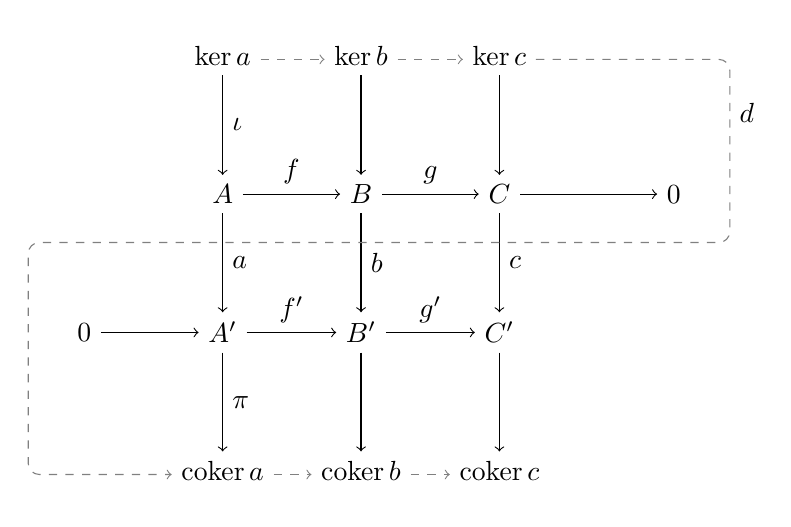
\begin{tikzpicture}
\matrix[matrix of math nodes,column sep={50pt,between origins},row sep={50pt,between origins},nodes={anchor=center}] (s)
{
&|[name=ka]| \ker a &|[name=kb]| \ker b &|[name=kc]| \ker c \\
%
&|[name=A]| A &|[name=B]| B &|[name=C]| C &|[name=01]| 0 \\
%
|[name=02]| 0 &|[name=A']| A' &|[name=B']| B' &|[name=C']| C' \\
%
&|[name=ca]| \coker a &|[name=cb]| \coker b &|[name=cc]| \coker c \\
};
\draw[->] (ka) edge node[auto] {\(\iota\)} (A)
          (kb) edge (B)
          (kc) edge (C)
          (A) edge node[auto] {\(f\)} (B)
          (B) edge node[auto] {\(g\)} (C)
          (C) edge (01)
          (A) edge node[auto] {\(a\)} (A')
          (B) edge node[auto] {\(b\)} (B')
          (C) edge node[auto] {\(c\)} (C')
          (02) edge (A')
          (A') edge node[auto] {\(f'\)} (B')
          (B') edge node[auto] {\(g'\)} (C')
          (A') edge node[auto] {\(\pi\)} (ca)
          (B') edge (cb)
          (C') edge (cc)
;
\draw[->,gray,dashed] (ka.mid east) -- (kb.mid west);
\draw[->,gray,dashed] (kb.mid east) -- (kc.mid west);
\draw[->,gray,dashed] (ca.mid east) -- (cb.mid west);
\draw[->,gray,dashed] (cb.mid east) -- (cc.mid west);

\draw[->,gray,rounded corners,dashed] (kc.mid east) -| 
  node[auto,text=black,pos=.7] {\(d\)} ($(01.east)+(.5,0)$)
 |- ($(B)!.35!(B')$) -| ($(02.west)+(-.5,0)$) |- (ca.mid west);
\end{tikzpicture}
\end{figure}

where the $\iota$ are the natural inclusion morphisms of the kernel and the $\pi$ are the natural projection morphisms.


\bigskip
\bigskip
\begin{proof}
\textbf{Morphisms between the kernel}

First we define the morphisms between the kernel. For example we define the map \[\bar{f}: \ker a \rightarrow \ker b\] by \[x \mapsto f(x).\] This is well defined, since \[b(f(x))=f'(a(x))=f'(0)=0,\] meaning that indeed $f(x) \in \ker b$. Of course, the upper left square then commutes and $\bar{f}$ is a homomorphism of $R$-modules. 

Of course, $\bar{g}: \ker b \rightarrow \ker c$ is defined analogously. 

\textbf{Morphisms between the cokernel}

We proceed to define the morphisms between the cokernel. Here we, for example, define the map \[\bar{f'}:\coker a \rightarrow \coker b\] by \[[y] \mapsto [f'(y)]\]

for $y$ in $A'$. Again we check that this gives us a well defined map: 

Let $y_1,y_2$ be in $A'$ with $[y_1]=[y_2]$. This means that $y_1-y_2 \in \im a$, therefore we have $z$ in $A$, such that $a(z)=y_1 - y_2$. Then \begin{align*}\bar{f'}([y_1])-\bar{f'}([y_2]) &= \bar{f'}([y_1-y_2])=[f'(y_1-y_2)] \\&= [f'(a(z))] = [b(f(z))] = 0 \end{align*} thus $\bar{f'}[y_1] = \bar{f'}[y_2]$. Here we have already used the homomorphism property of $\bar{f'}$ that needs a quick proof:
%
% 
\begin{align*} 
	\bar{f'}([x]+[y]) &=\bar{f'}([x+y])=[f'(x)+f'(y)]\\
	&=[f'(x)]+[f'(y)]=\bar{f'}([x])+\bar{f'}([x])\\[0.5em]
	\bar{f'}(r[x])&=\bar{f'}([rx])=[f'(rx)]=r[f'(x)]=r\bar{f'}([x]) 
\end{align*}
%
%
for $r \in R$. Of course, the lower left square commutes, in fact, the way we defined $\bar{f'}$ was the only chance to have it commute.

Again we use an analogous construction to obtain the morphism \[\bar{g'}: \coker b \rightarrow \coker c. \]

\textbf{The morphism \boldmath $d: \ker c \rightarrow \coker a$} \unboldmath

Now we define the morphism $d: \ker c \rightarrow \coker a$. Starting with an element $x \in \ker c$, we chase $x$ through the diagram until we arrive in $\coker a$: 

First we obviously want to map $x$ to $\iota(x) \in C$ and then use the surjectivity of $g:B \rightarrow C$ to get an (not necessarily unique) element $y$ in $B$, such that $g(b)=\iota(x)$. We then take $b(y) \in B'$ and from \[g'(b(y))=c(g(y))=c(\iota(x))=0,\] we use the exactness of the lower rower to obtain a unique(!)  element $z$ in $A'$, with $f'(z)=b(y)$. With $\pi(z)$ we finally arrive in $\coker a$. 

We now immediately want to define $d$ as \[d: \ker c \rightarrow \coker a,\ x \mapsto \pi(z),\] however, we first need to show that this way, this gives a well-defined map.

For this take $y_1$ and $y_2$ in $B$, with \[g(y_1)=g(y_2)=\iota(x).\] We want to show that this gives the same element $\pi(z)$ in $\coker a$. Since $y_2-y_1 \in \ker g$, we have a $w \in \ker g$ such that $y_2= y_1 + w$. Using the exactness of the upper row we can rewrite this as \[y_2 = y_1 + f(u)\] with $u \in A$.

 We then have \[ z_1 = f'^{-1}(b(y_1)) \ \mathrm{and} \ z_2=f'^{-1}(b(y_2))\] as the elements of $A'$ the result from chasing $y_1$ and $y_2$ to $A'$ and compute \begin{align*}z_2&=f'^{-1}(b(y_2))=f'^{-1}(b(y_1 + f(u)) \\ &=f'^{-1}(b(y_1)) + f'^{-1}(b(f(u))) \\ &= z_1 + f'^{-1}(f'(a(u))) = z_1 + a(u) \end{align*} (mind the injectivity of $f'$), giving us \[\pi(z_2)= \pi(z_1) + \pi((a(u)) = \pi(z_1)\] as desired.
 
Again, $d$ was the only choice to make the diagram commute,  we now to need to ascertain that $d$ is morphism of $R$-modules. 

Taking $x_1 + x_2 \in \ker c$, we have $\iota(x_1)+\iota(x_2) \in C$ and since d is well defined, we may take $y_1 + y_2 \in B$, where $b(y_i)=\iota(x_i)$,$i=1,2$, as the pre-image. Then the pre-image of $b(y_1)+b(y_2)$ clearly is $z_1 + z_2$, where $f'(z_i)=b(y_i)$,$i=1,2$ and finally obtain $\pi(z_1) + \pi(z_2)$ for $d(x_1+x_2)$, thus \[d(x_1 + x_2)=d(x_1)+d(x_2).\]

For $rx \in \ker c$, $r \in R$, the argumentation is completely analoguous: 

\end{proof}

\bigskip 

\normalfont We now want to use the snake lemma to show the existence of the long exact homology sequence:

\bigskip

\itshape Given a short exact sequence of chain complexes \[\xymatrix@=0.7cm{0 \ar[r] & A_{\bullet} \ar[r] & B_{\bullet} \ar[r] & C_{\bullet} \ar[r] & 0} \] there is a long exact sequence \[\xymatrix@=0.6cm{\hdots \ar[r] & H_{n+1}(C) \ar[r] & H_n(A) \ar[r] & H_n(B) \ar[r] & H_n(C) \ar[r] & H_{n-1}(A) \ar[r] & \hdots} \]

\end{document}